\documentclass[11pt, a4paper]{article}
% \usepackage[T1]{fontenc}
\usepackage[utf8]{inputenc}
\usepackage{listings}
\usepackage[margin=1.0in]{geometry}
\usepackage{color}
\usepackage{graphicx}
\usepackage{tabularx}
\usepackage{url}
\usepackage[normalem]{ulem} 
\usepackage{enumitem}

\title{Rock the net}
\author{Elias Frantar, Samuel Schmidt, Nikolaus Schrack, Gary Ye}
\date{\today{}, Wien}
\begin{document}

\lstset{ %
  backgroundcolor=\color{white},   % choose the background color; you must add \usepackage{color} or \usepackage{xcolor}
  basicstyle=\footnotesize,        % the size of the fonts that are used for the code
  breakatwhitespace=false,         % sets if automatic breaks should only happen at whitespace
  breaklines=true,                 % sets automatic line breaking
  captionpos=b,                    % sets the caption-position to bottom
% commentstyle=\color{mygreen},    % comment style
  deletekeywords={...},            % if you want to delete keywords from the given language
  escapeinside={\%*}{*)},          % if you want to add LaTeX within your code
  extendedchars=true,              % lets you use non-ASCII characters; for 8-bits encodings only, does not work with UTF-8
% frame=single,                    % adds a frame around the code
  keepspaces=true,                 % keeps spaces in text, useful for keeping indentation of code (possibly needs columns=flexible)
% keywordstyle=\color{blue},       % keyword style
% language=bash,                   % the language of the code
  morekeywords={*,...},            % if you want to add more keywords to the set
  numbers=left,                    % where to put the line-numbers; possible values are (none, left, right)
  numbersep=5pt,                   % how far the line-numbers are from the code
  rulecolor=\color{black},         % if not set, the frame-color may be changed on line-breaks within not-black text (e.g. comments (green here))
  showspaces=false,                % show spaces everywhere adding particular underscores; it overrides 'showstringspaces'
  showstringspaces=false,          % underline spaces within strings only
  showtabs=false,                  % show tabs within strings adding particular underscores
  stepnumber=1,                    % the step between two line-numbers. If it's 1, each line will be numbered
  tabsize=2,                       % sets default tabsize to 2 spaces
  title=\lstname                   % show the filename of files included with \lstinputlisting; also try caption instead of title
}


\maketitle
\newpage
\tableofcontents
\newpage

\section{Task description}

\subsection{Basic Tasks}
Implement a simple-to-use application to monitor and configure a hardware firewall appliance “Juniper NetScreen 5GT “. The firewall allows read access over the SNMP-protocol (your app should be able to test if SNMPv3 is available and if not fallback on SNMPv2c) and write access over Telnet.
\\\\
Your app should accomplish following tasks:
\begin{itemize}
\item List all configured firewall rules (policies) on the device, add the details of the mentioned services and zones as well.
\item Allow refreshing of the list by clicking a button and by a configurable time-intervall. Your GUI should remain responsive even with short refresh-intervals!
\item Visualize the thru-put for a highlighted firewall-rule (nice2have: multiple rows) in a line-chart (configurable refresh-interval, unit bytes/sec)
\item Encapsulate the data retrieval for further reuse and easy expansion. An UML-model of your design will help you defend it at the review!
\item Build a visual appealing and easy to use interface (there is more than Swing out there).
\end{itemize} 

\subsection{Additional Tasks}
\begin{itemize}
\item Since there is only one firewall-appliance available, the time each team can test with the hardware will be strictly limited. Therefore it is essentially to use mock-objects to allow testing the app during times where the hardware is not available.
\item An additional benefit of using mock-objects will be, that a CI-Server can use them for automated building and testing.
\item You only need to consider firewall-rules for TCP and UDP connections in IPv4.
\item You can find Information about the SNMP-Mibs special for the manufacturer of the used appliance here (maybe not all of the Mibs work with the used model): 
\item http://www.oidview.com/mibs/3224/md-3224-1.html
For exploring the SNMP-Data coming from the appliance you can use tools like this:
\item http://ireasoning.com/mibbrowser.shtml
\end{itemize} 

\subsection{Advanced tasks (obligatory for grades better than B3)}
Additionally to the basic tasks your app should accomplish the following:
\begin{itemize}
\item Alarm the user visually and per email if the config of the firewall-rules changes. To avoid polling use the SNMP-trap mechanism.
\item Allow managing of firewall-rules (CRUD). To accomplish this, you will have to send configuration commands via telnet or ssh. An admin-account is available per request.
\item Use multicast-groups to build a simple transaction system to serialize administrative tasks on the firewall (for example pass an “admin token” to recognize the collaborator who is all    owed to write to the firewall). This should also work in a heterogenous environment (different implementations, different OSes), so you have to coordinate with other teams.
\item Make sure, that your interface to the firewall allows an easy change of the firewall-model (new releases, manufacturer, ...). It is not necessary to make this configurable in the GUI but must (explicitly) be considered in your software-design!
\end{itemize} 

\subsection{Teams}
Build teams with 3 to 5 participants (5 only if two or more members choose advanced level and at least one member chooses basic level). Each individual team-member has to implement, test and document code and is allowed to choose the level of difficulty he/she wants to achieve. For example: if you have a group of four students and two of them want to achieve advanced level, they can focus their implementation work on the advanced tasks. The other two team-members focus on the basic functionality. In any case there must be a working product, advanced tasks can not stand for themselves.

\subsection{Grading}
A team can apply for submission with a (mostly) functional product.
Each team-member will be graded separately, based on the documentation (and git-logs) which name him/her as author in all three main competencies as listed.
Advanced tasks will only be considered if the basic tasks are fulfilled for the most part in this team.

\subsection{Submission}
\begin{itemize}
\item Every group must have its own design/solution! Meta-group solutions will end in massive loss of points!
\item As for group work usual, a protocol with the UML-Design, the work-sharing, the timetable and test documentation is mandatory!
\item Upload your solution as a ZIP file. Please submit only the sources of your solution and a build file (build.xml, pom.xml, Makefile etc.) not the compiled class files and only approved third-party libraries. \item Your submission must compile and run!
\item Before the submission deadline, you can upload your solution as often as you like. Note that any existing submission will be replaced by uploading a new one.
\end{itemize}

\newpage

\section{Effort estimation}
\subsection{Basic Tasks}
\begin{tabular} {| l | c | c | c |} \hline
Task &	Original Estimate & Remaining Estimate & Time spent \\ \hline
Preparation for the Tasks &	20 &	0.00 & 24.50 \\ \hline
Listing firewall rules &	7 &	2 &	9.50 \\ \hline
Refreshing rules &	6 &	6 &	0.00 \\ \hline
Visualize thru put & 8 &	4 &	5.00 \\ \hline
Encapsulate the data retrieval &	4	& 0.00 &	4.00 \\ \hline
GUI	 & 10 &	7 &	8.00 \\ \hline
Final Documentation  &	8	& 2	& 5.00 \\ \hline
Basic Total	& 63 &	31.00 &	56.00 \\ \hline
\end{tabular}

\subsection{Advanced Tasks}
\begin{tabular} {| l | c | c |}\hline
Task &	Original Estimate & Time spent \\ \hline
Alarm the user &	7	& 0 \\ \hline
Firewall rules CRUD &	6 & 	0 \\ \hline
Transactions by Multicast &	8  &	0 \\ \hline
Exchangeable & 5 & 2 \\ \hline
Advanced Total & 26 &	2 \\ \hline
\end{tabular}

\subsection{Total}
\begin{tabular} {| l | c | c |}\hline
	Task &	Original Estimate & Time spent \\ \hline
	Total & 89 & 142 \\ \hline
\end{tabular}

\newpage

\section{Work Sharing}

\subsection{Original Tasks}

\textbf{Elias Frantar}
\begin{enumerate}[noitemsep]
	\item SNMP-Connections: design, implementation, testing, documentation
	\item SSH-Connection: design, implementation, testing, documentation
	\item GUI/Controller programming: implementation, documentation
\end{enumerate}

\noindent \textbf{Samuel Schmidt}
\begin{enumerate}[noitemsep]
	\item GUI/Controller: design, implementation, documentation
	\item SNMP-hook: design, implementation, testing, documentation
	\item Notifications (email, pop-ups): design, implementation, testing, documentation
\end{enumerate}

\noindent \textbf{Nikolaus Schrack}
\begin{enumerate}[noitemsep]
	\item Thru put graph: design, implementation, testing, documentation
	\item Data refreshing: design, implementation, testing, documentation
	\item Automated GUI-testing
\end{enumerate}

\noindent \textbf{Gary Ye}
\begin{enumerate}[noitemsep]
	\item Data mapping: design, implementation, testing, documentation
	\item CRUD: design, implementation, testing, documentation
	\item CI server
	\item Multicast-Group-Transactions: design, implementation, testing, documentation
\end{enumerate}

\subsection{Time Spent}
\begin{tabular} {| l | c | c | c | c | c |} \hline

	Task 								& 	Frantar 	& 	Schmidt 	& 	Schrack 	& 	Ye 		& 	Total 	\\ \hline \hline
	
	Preparation							& 	9			&				&				&	11.5	&			\\ \hline
	Documentation						&	7			&				&				&	9.5		&			\\ \hline
	Model Design						& 	2			&				&				& 	10		&			\\ \hline
	Continuous Integration				& 	0			& 				& 				&	9.5		&			\\ \hline \hline
		
	GUI									& 	2			&				&				& 	0		&			\\ \hline
	SNMP-connections					& 	11			&				&				& 	0		&			\\ \hline
	Thru-put graph						& 	1			&				&				& 	1.75	&			\\ \hline
	Data retrieval and mapping			& 	0			&				&				& 	2		&			\\ \hline
	Information refreshing				&	3			&				&				&	0		&			\\ \hline
	Rule-table with graph selection		&	2			&				&				&	0		&			\\ \hline \hline
	
	SNMP-Trap							&	0			&				&				&	0		&			\\ \hline
	Emails and notifications			&	1			&				&				&	0		&			\\ \hline
	SSH-connection						&	8			&				&				&	0		&			\\ \hline
	CRUD								& 	3			& 				& 				&	15		&			\\ \hline
	Multicast Groups					&	0			&				&				&	4		&			\\ \hline \hline
	
	Total								&	49			&				&				&	63.25	&			\\ \hline
	
\end{tabular}

\newpage


\section{Grade of Completion}

The following user-stories have been deduced from the task description. All not crossed out ones have been successfully implemented and are included in the final product. \\
In summary everything except Multi-Cast-Groups and the SNMP-trap is working satisfyingly.
\\\\
Crossed out ones did not fully work and therefore are not included in the final product. See section~\ref{sec:problems} for more information on the problems we had.

\vspace{10pt}
\noindent \textbf{Basic tasks:}
\begin{itemize}
\item As a user, I want to connect to my firewall device by entering its IP-address.
\begin{itemize}
\item As a user, I want to connect with SNMPv2c.
\item As a user, I want to connect with SNMPv3.
\end{itemize}
\item As a user, I want a visually appealing graphical user interface.
\item As a user, I want to list all firewall-rules configured on my device.
\begin{itemize}
\item As a user, I want to see the port of a firewall rule.
\item As a user, I want to see the zone of a firewall rule.
\item As a user, I want to see the service of a firewall rule.
\item As a user, I only want to see the TCP and UDP firewall rules.
\end{itemize}
\item As a user, I want the rules to be refreshed.
\begin{itemize}
\item \sout{As a user, I want the rules to be refreshed automatically.}
\begin{itemize}
\item As a user, I want to configure the refresh intervals.
\end{itemize}
\item As a user, I want to refresh the rules manually by pressing on a button.
\end{itemize}
\item As a user, I want to visually monitor the thru-put of a firewall-rules.
\begin{itemize}
\item As a user, I want to visually see the thru-put in line-chart.
\item As a user, I want to monitor multiple rules at the same time.
\end{itemize}
\item As a developer, I want the data retrieval to be encapsulated for further reuse and expansion.
\end{itemize}
\noindent \textbf{Advanced tasks:}
\begin{itemize}
\item \sout{As a user, I want to be notified if a rule has been changed without my assistance.}
\begin{itemize}
\item As a user, I want to be notified by a pop-up window.
\item As a user, I want to be optionally notified by email.
\item As a user, I want to configure my email-address.
\begin{itemize}
\item As a user, I want to configure the email-address in the GUI.
\end{itemize}
\end{itemize}
\item As a user, I want to configure all firewall-rules on the device.
\begin{itemize}
\item As a user, I want to create a fully new rule.
\item As a user, I want to fully edit an existing rule.
\item As a user, I want to delete an existing rule.
\item As a user, I want to login before editing a rule.
\begin{itemize}
\item As a user, I want to stay logged in for the whole session after I have logged in for the first time.
\end{itemize}
\end{itemize}
\item \sout{As a user, I want to have a transaction system for write access on the firewall, so that no editing conflicts can occur when multiple applications are trying to modify at the same time.}
\item As a developer, I want to be able to easily modify the software so that it works with other firewall hardwares.
\begin{itemize}
\item As a developer, I only want to exchange the SNMP-commands to make the application work with other firewall hardwares.
\end{itemize}
\end{itemize}

\section{Design}

\subsection{UML Diagram}
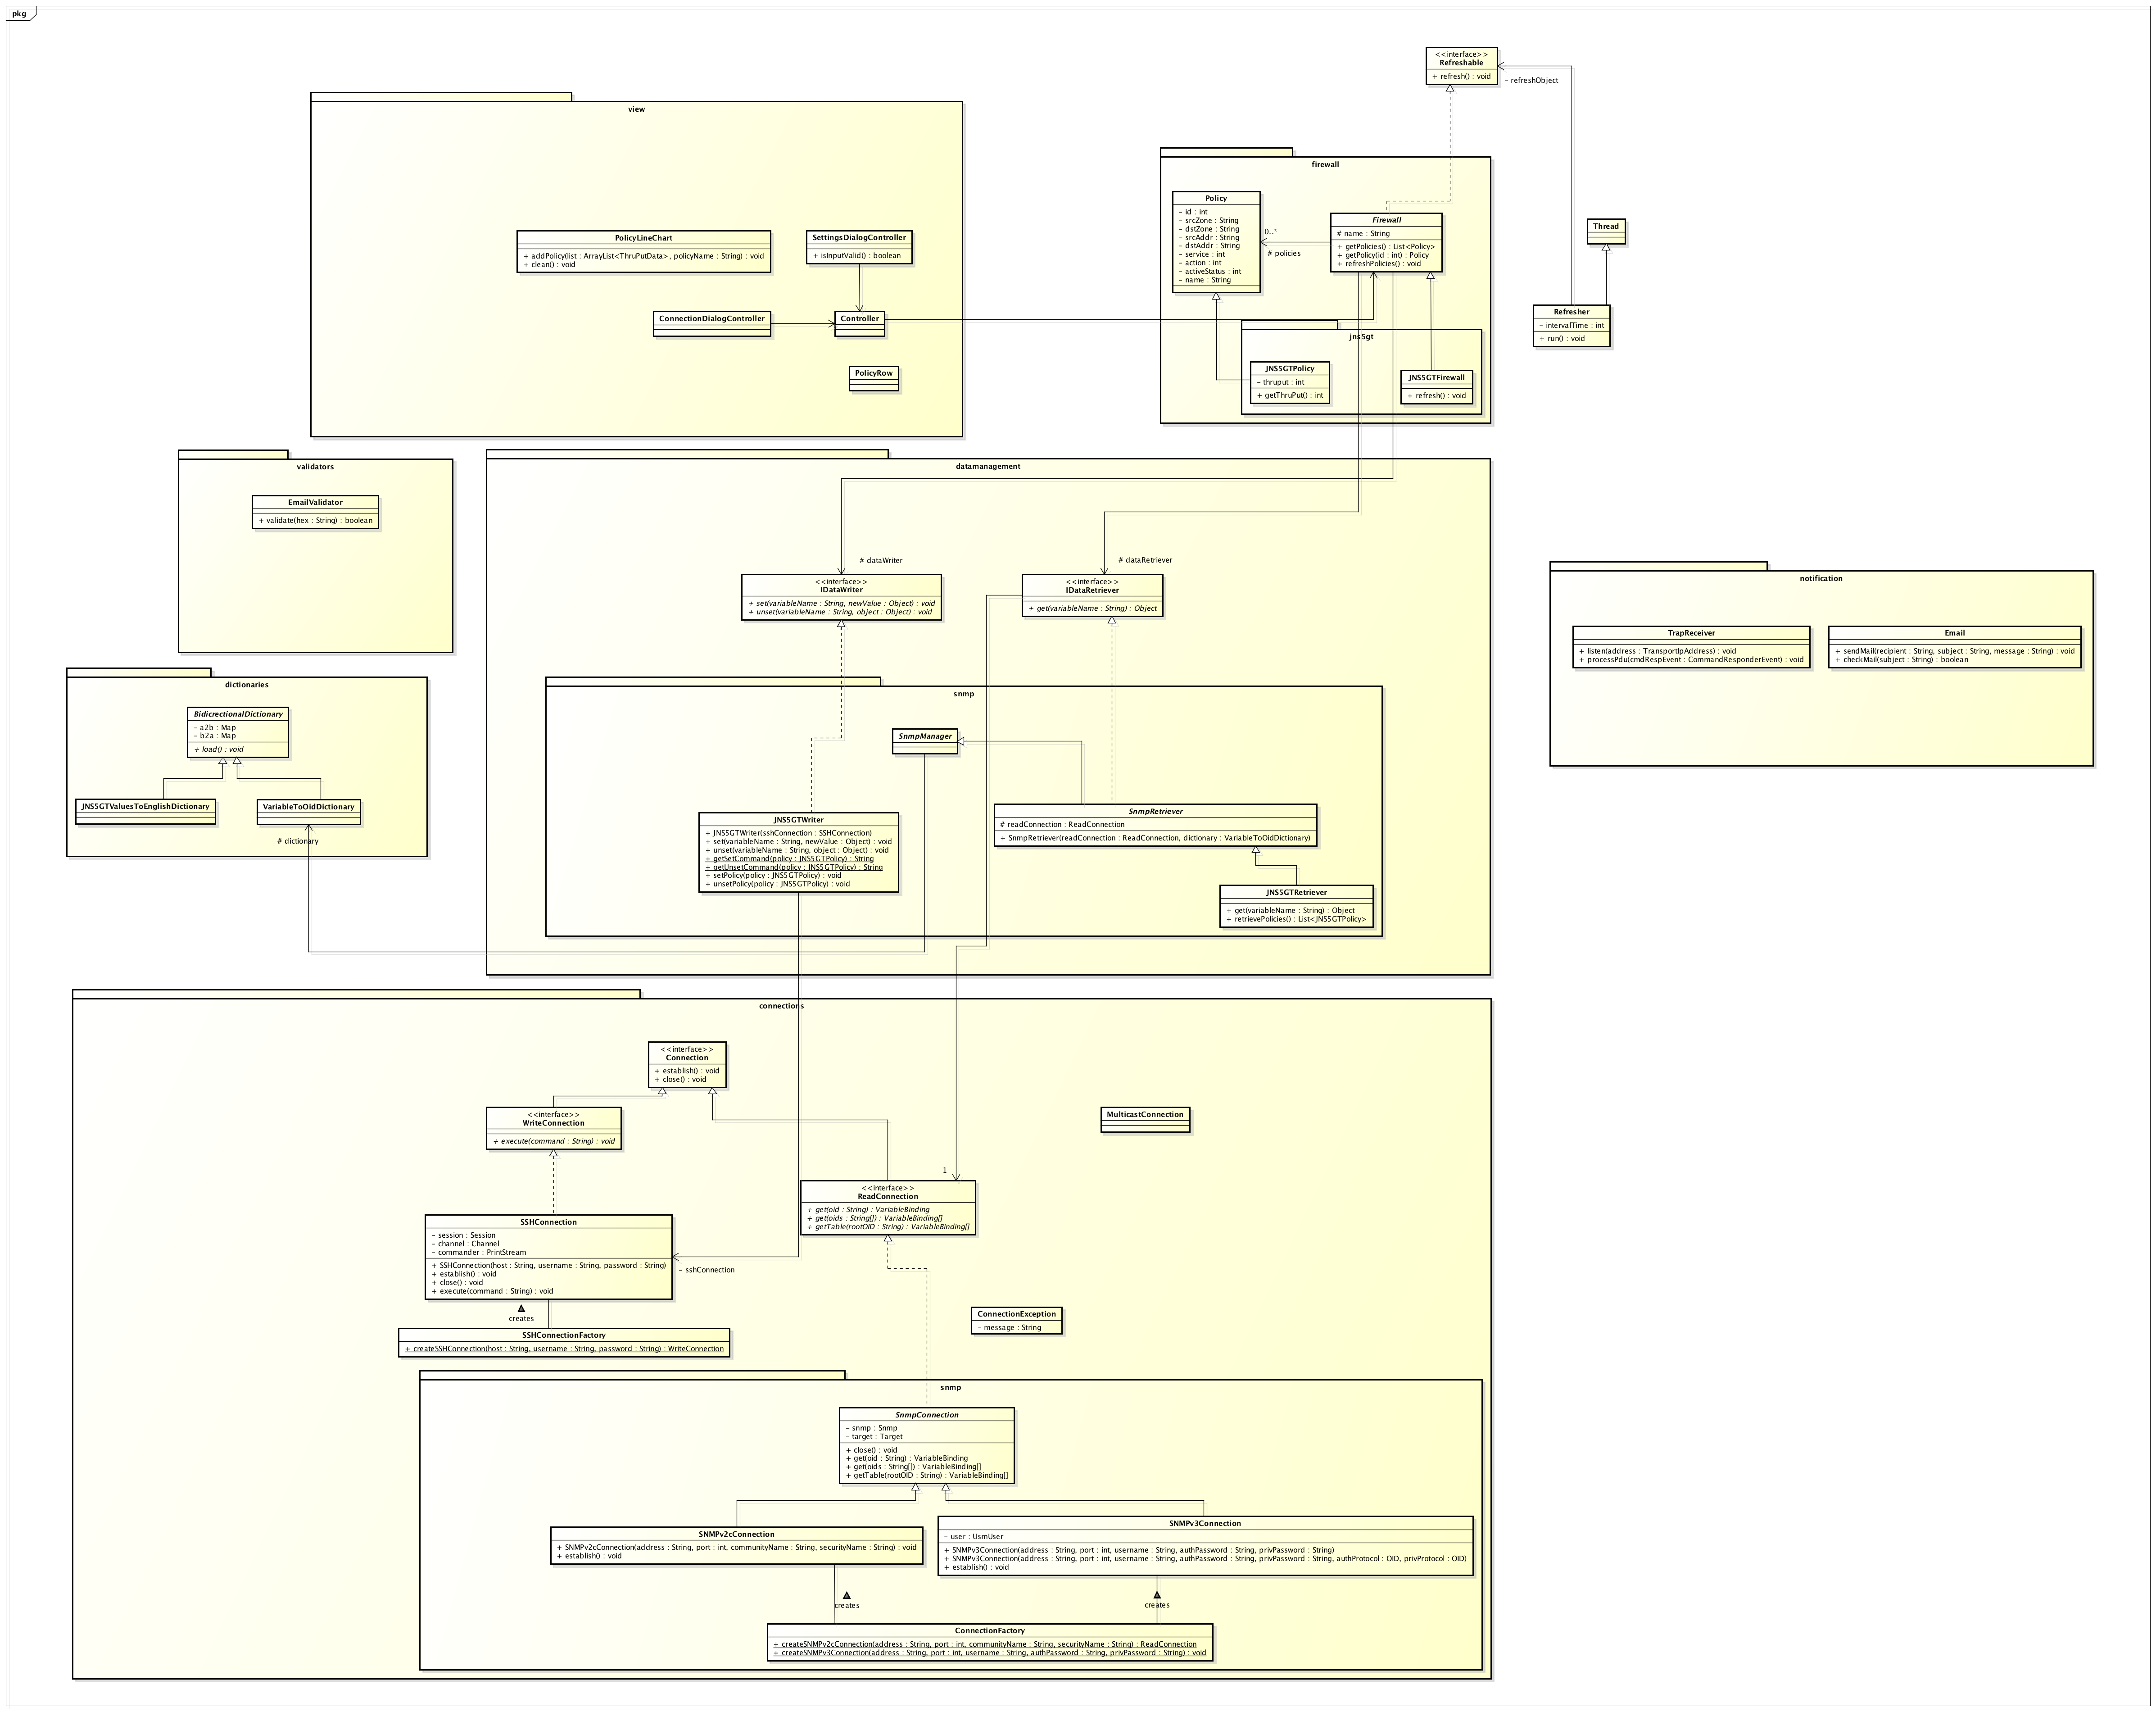
\includegraphics[width=\textwidth]{images/umlv3}

\newpage

\section{Installation and Preparation}

For starting up the program one does only need to have the build tool \textit{ant}. 

The important tasks of the ant build script is listed here:

\section{Test report}

Testing was categorized in three sub categories:

\begin{itemize}
	\item Unit Tests
	\item Exception Handling
	\item Graphical User Interface Tests
\end{itemize}

\subsection{Unit Tests}

Unit tests were mainly done in the model classes. The following figure is a snippet of the latest coverage report (October 31st) created in Jenkins. 

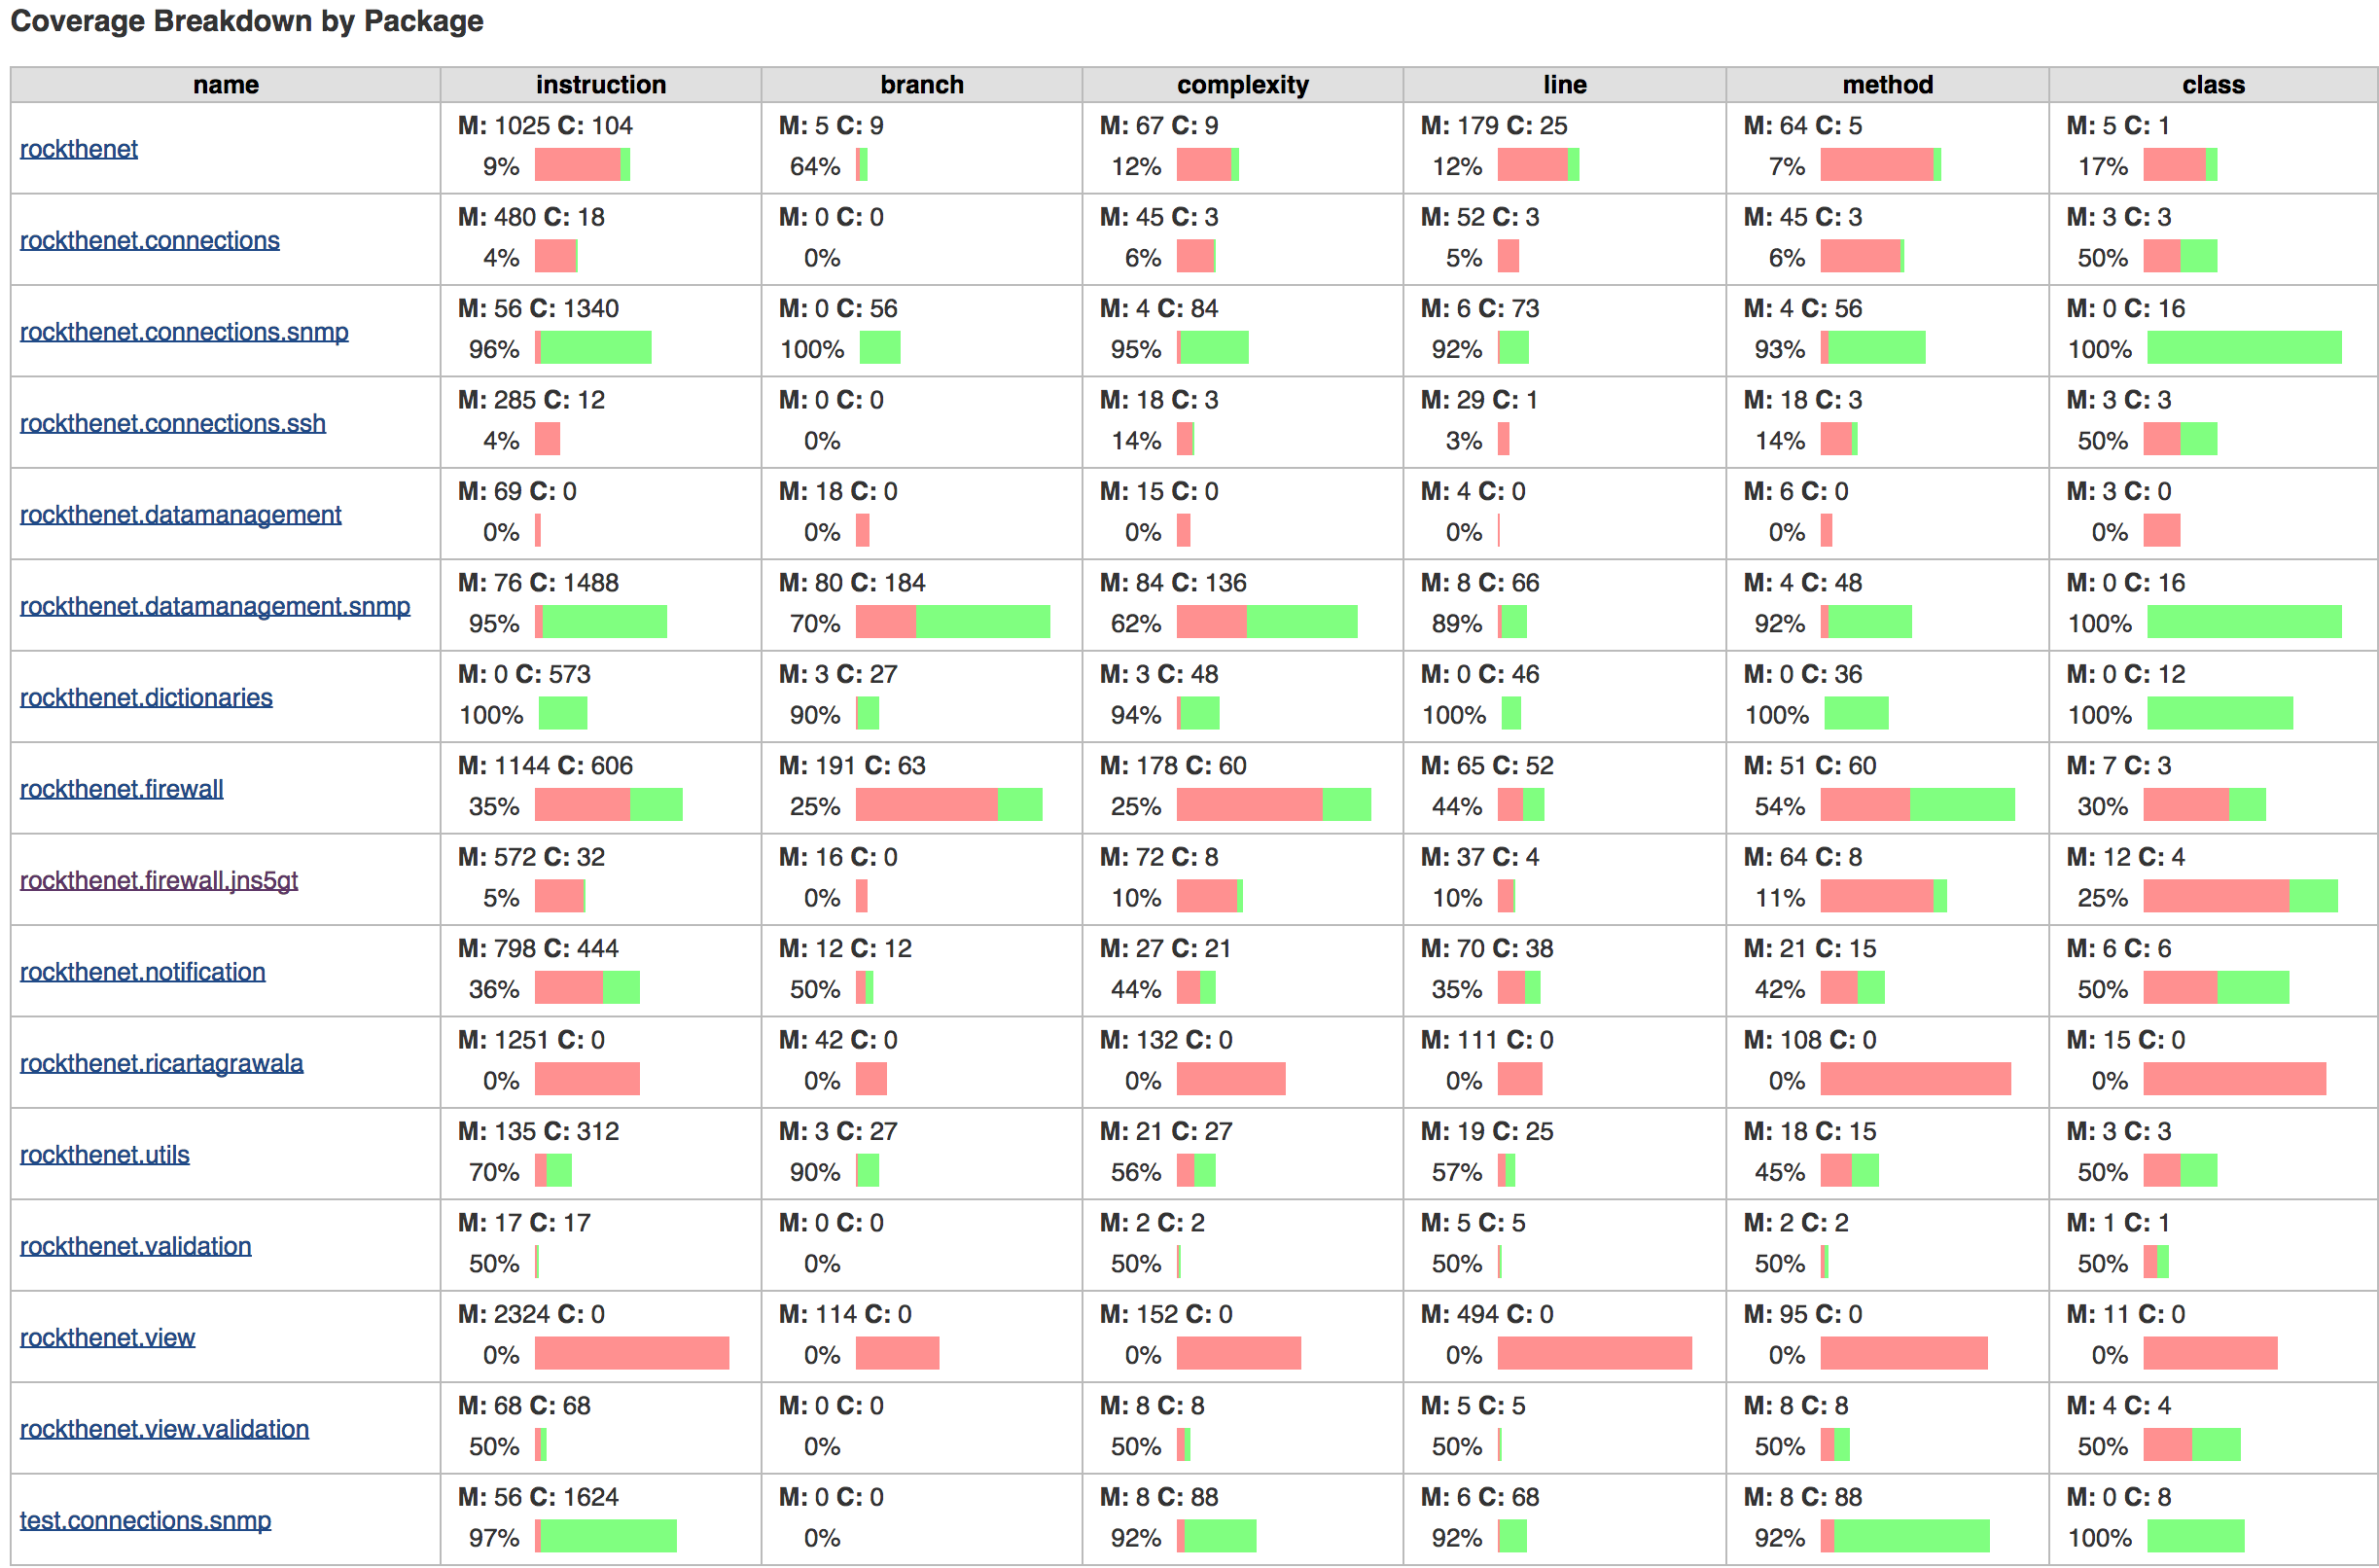
\includegraphics[width=\textwidth]{images/coverage}

The tests of the \lstinline|view| package have zero coverage because it was tested in a different way. Some of the packages also have zero coverage due to very simple get and set methods, which are unnecessary to test.  

\subsection{Exception Handling}
% TODO: You are never strong enough that you don't need help.”  ― César Chávez
\subsection{GUI Test}
% TODO: NIKO?

\section{Occurred problems}
\label{sec:problems}
\subsection{Multicast Connection}

Multicast connection couldn't be tested because of a very nasty and yet unresolved bug. This has been a major issue for weeks and no solutions could be found in the Internet. 
\\\\
In fact it wasn't even possible to create a Multicast-group manually on some of the team-members PCs.

Concretely the following code throws an exception that cannot be resolved. 

\begin{lstlisting}
InetAddress group = InetAddress.getByName("224.0.0.1");
int port = 6667;

peer1 = new Peer(new MulticastConnection(group, port));
peer1.connect();
\end{lstlisting}

The exception is as follows:

\begin{lstlisting}
java.net.SocketException: Can't assign requested address
at java.net.PlainDatagramSocketImpl.join(Native Method)
at java.net.AbstractPlainDatagramSocketImpl.join(AbstractPlainDatagramSocketImpl.java:178)
at java.net.MulticastSocket.joinGroup(MulticastSocket.java:323)
at rockthenet.connections.MulticastConnection.establish(MulticastConnection.java:48)
at test.connections.MulticastConnectionTest.setup(MulticastConnectionTest.java:29)
at sun.reflect.NativeMethodAccessorImpl.invoke0(Native Method)
at sun.reflect.NativeMethodAccessorImpl.invoke(NativeMethodAccessorImpl.java:62)
at sun.reflect.DelegatingMethodAccessorImpl.invoke(DelegatingMethodAccessorImpl.java:43)
at java.lang.reflect.Method.invoke(Method.java:483)
at org.junit.runners.model.FrameworkMethod$1.runReflectiveCall(FrameworkMethod.java:47)
at org.junit.internal.runners.model.ReflectiveCallable.run(ReflectiveCallable.java:12)
at org.junit.runners.model.FrameworkMethod.invokeExplosively(FrameworkMethod.java:44)
at org.junit.internal.runners.statements.RunBefores.evaluate(RunBefores.java:24)
\end{lstlisting}

That's why Ricart Agrawla couldn't be implemented successfully with a Multicast connection. 







\newpage

\section{Technologies}
\subsection{Mock-Objects}
\subsubsection{Setup}

\begin{enumerate}
	\item Download \textit{Mockito} from \cite{MockitoDownload}
	\item Add \textit{junit-4.11.jar} and \textit{mockito-all-1.9.5.jar} to the project's \textit{classpath}
	\item Done
\end{enumerate}

\subsubsection{How to use Mockito}

\textit{Mockito} allows you to mock interfaces, but also concrete classes, with a single line of code:
	
\begin{lstlisting} 
List mockedList = mock(List.class); // creates a mock-Object of `List` 
\end{lstlisting}
	
A \textit{Mockito-Mock-Objects} remembers all methods, which have been called. So you can check afterwards if some method has been called with some parameters.
	
\begin{lstlisting}
	mockedList.add("one");
	    
	verify(mockedList).add("one"); // test "successful" because that exact method with that exact parameter has been called before
	verify(mockedList).add("two"); // test "failed" because `.add("two")` has not been called before
\end{lstlisting}

One of the main functionalities of a Mock-object is that it can provide kind of dummy-methods, called *stubs*, i.e. when a specific method with a specific parameter is called, a specific
value is returned. There are also some kind of wildcards for the methods parameters, if you want to return "first" on any given Integer-parameter. That can be achieved like this:

\begin{lstlisting}
    when(mockedList.get(0)).thenReturn("first"); // `mockedList` will return "first" when `.get(0)` is called
    System.out.println(mockedList.get(0)); // prints "first"
    
    when(mockedList.get(anyInt()).thenReturn("any int"); // will return "any int" if you pass for example: 1, 27, 4, ...
    System.out.println(mockedList.get(2345)); // prints "any int"
\end{lstlisting}

You can also make the mock throw Exceptions by using `.thenThrow()` or make void methods throw Exceptions by:

\begin{lstlisting}
    doThrow(new RuntimeException()).when(mockedList).clear();
    mockedList.clear(); // throws RunTime-Exception
\end{lstlisting}

You can also verify how often a specific method has been called. That works like this:

\begin{lstlisting}
    mockedList.add("once");
    
    verify(mockedList, times(1)).add("once"); // success because `.add("once")` has been called exactly once
    verify(mockedList, times(2)).add("once"); // fails because it has only been called once
\end{lstlisting}

For \textit{times(0)}, you should better use \textit{never()}.
 
Like the number of invocations, you can also verify the order of of invocations:

\begin{lstlisting}
    mockedList.add("first");
    mockedList.add("second");
    
    InOrder inOrder = inOrder(mockedList);
    
    inOrder.verify(mockedList).add("first");
    inOrder.verify(mockedList).add("second");  
\end{lstlisting} 
    
For explanation of additional functionalities and full documentation, see \cite{MockitoDownload}.

\subsection{Java FX}
Java 8 supports Java FX, so no further installation will be needed if Java 8 is used. 

\subsubsection{Line Charts}

For the application a line chart has been needed. Using the LineChart class it is possible to show up a pretty visual appealing line chart which updates with or without animation.

A sample picture of the Java FX LineChart is shown below. 

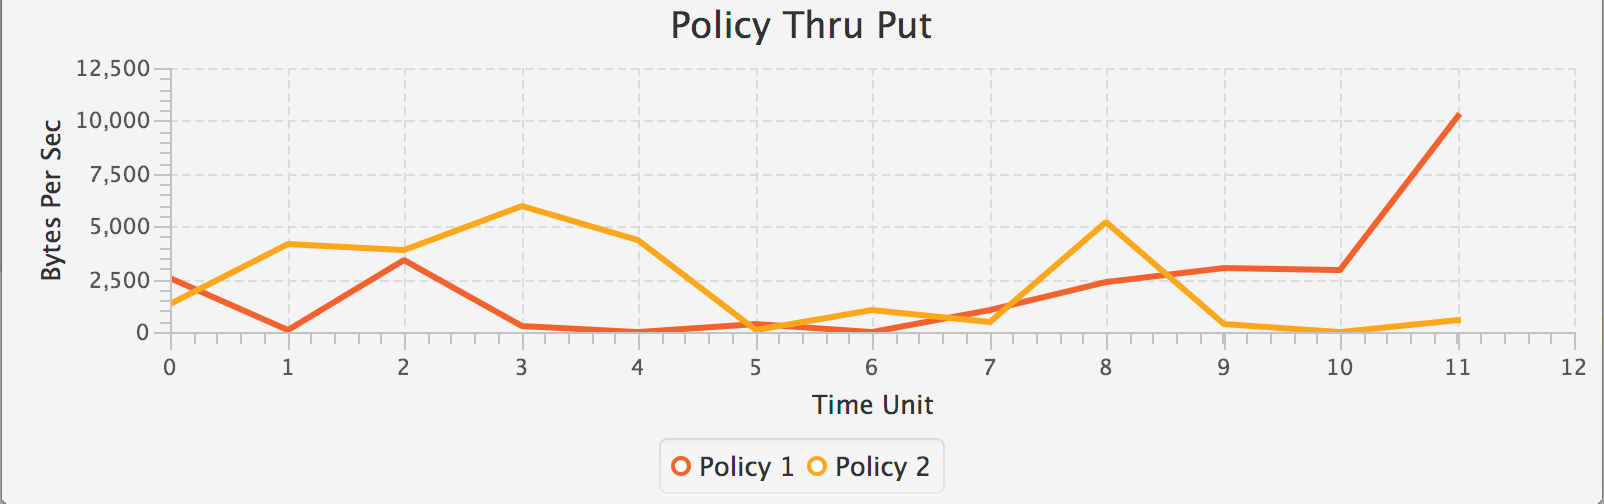
\includegraphics[width=\textwidth]{images/linechart.png}

% http://docs.oracle.com/javafx/2/charts/line-chart.htm#CIHGBCFI

\subsection{SNMP - Simple Network Management Protocol}

It is, like the name says, a simple network protocol to manage and monitor the devices in a network. Practically, the monitored devices are all connected to a central system that controls them by using the “Simple Network Manager Protocol”.

\begin{figure}[h!]
	\centering
	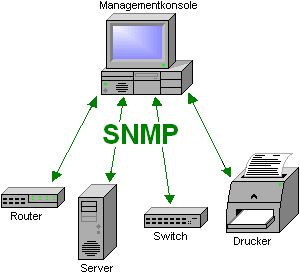
\includegraphics[width=0.6\textwidth]{images/SNMP-Managementkonsole.png}
	\caption{The Router, the Server, the Switch and the Printer are connected via the SNMP to the management system.}
\end{figure}


% (Source: http://de.wikipedia.org/wiki/Simple_Network_Management_Protocol)

\subsubsection{SNMPv2c and SNMPv3 differences}

With v3 no changes to the protocol aside from added security and remote configuration enhancements to SNMP were added. However new textual conventions, concepts and terminology were introduced.

The core Snmp class documentation \cite{SNMP4JDoc} offers only insight on big differences in SNMPv1(asynchronous) and v3(synchronous) implementations. TransportMapping only affects UDP/TCP/… configurations.

\subsection{MIB - Management Information Base}
As the management system wants to read data from a device, it has to know how the structure of the data storage. The specified informations can be retrieved from the corresponding MIB. 

The MIB of the device, that is being used for this exercise, can be found from \cite{MIBDownload}.

The MIB is structured like a tree (examples can be found in the Wikipedia article). Every object of the device can be identified by the OID (Object Identifier), which is just a list of numbers separated by a dot.

One can for example GET/SET the variables by using the OI of the specified object.

Also one can use a MIB browser to explore the structure \cite{MIBBrowser}.
\subsection{Multicast-Groups}

Multicast is basically a group communication where the packages are sent only once and arrive at their destination simultaneously. The nodes of the network (router, switches) will take care of how the messages will be distributed. So the sender does not have to worry about the number of receivers.

The most common protocol for this is UDP, even though it’s unreliable. There exists also reliable protocols where loss detection and retransmission are provided.

In the Java API there exists a class which provides multicasting \cite{javamulticast}. The documentation itself says:
“A multicast group is specified by a class D IP address and by a standard UDP port number. Class D IP addresses are in the range 224.0.0.0 to 239.255.255.255, inclusive. The address 224.0.0.0 is reserved and should not be used.”

A code snippet has also been provided:

\begin{lstlisting}
// join a Multicast group and send the group salutations
...
String msg = "Hello";
InetAddress group = InetAddress.getByName("228.5.6.7");
MulticastSocket s = new MulticastSocket(6789);
s.joinGroup(group);
DatagramPacket hi = new DatagramPacket(msg.getBytes(), msg.length(),
group, 6789);
s.send(hi);
// get their responses!
byte[] buf = new byte[1000];
DatagramPacket recv = new DatagramPacket(buf, buf.length);
s.receive(recv);
...
// OK, I'm done talking - leave the group...
s.leaveGroup(group);
\end{lstlisting}

The important methods of the MulticastSocket class are:
\begin{description}
\item[joinGroup] to join the given group
\item[receive] receive the message of the subscribed group
\item[leaveGroup] leave the specified group
\end{description}

\subsection{Juniper Netscreen 5GT}

Juniper Netscreen 5GT has proprietary configuration commands for its own operating system. When establishing an SSH or Telnet connection with the firewall, the user will automatically obtain access for configuring the firewall. Some of those commands will be described in this section. 

\begin{lstlisting}
set policy id <id> name <policy-name> from <src-zone> to <dst-zone> <src-addr> <dst-addr> <service> [permit | deny]
\end{lstlisting}

For overwriting policies we only have to execute the command above like we are adding the new rule. The only thing we need to care about is the id of the corresponding policy that should be changed. 

For removing firewall rules we need to do the contrary of setting - \textit{unsetting}.

\begin{lstlisting}
unset policy id <id> 
\end{lstlisting}


\subsection{Continuous Integration Server}

For this project Jenkins was installed on a Ubuntu Server. The instructions from the official Jenkins documentation \cite{jenkins:ubuntu} were followed and documented. 

Installing Jenkins can be easily installed by entering the following commands: 

\begin{lstlisting}
wget -q -O - https://jenkins-ci.org/debian/jenkins-ci.org.key | sudo apt-key add -
sudo sh -c 'echo deb http://pkg.jenkins-ci.org/debian binary/ > /etc/apt/sources.list.d/jenkins.list'
sudo apt-get update
sudo apt-get install jenkins 
\end{lstlisting}

Then we should use Jenkins on Port 80 by installing apache and doing the following:

\begin{lstlisting}
sudo apt-get install apache2
sudo a2enmod proxy
sudo a2enmod proxy_http
sudo a2dissite default
sudo a2dissite default
\end{lstlisting}

Create /etc/apache2/sites-available/jenkins and fill with:
\begin{lstlisting}
<VirtualHost *:80>
	ServerAdmin webmaster@localhost
	ServerName ci.company.com
	ServerAlias ci
	ProxyRequests Off
	<Proxy *>
		Order deny,allow
		Allow from all
	</Proxy>
	ProxyPreserveHost on
	ProxyPass / http://localhost:8080/ nocanon
	AllowEncodedSlashes NoDecode
</VirtualHost> 
\end{lstlisting}


Now enter the following commands. 

\begin{lstlisting}
sudo a2ensite jenkins
sudo apache2ctl restart
\end{lstlisting}


Under "Manage Jenkins" and "Configure System" we can find the basic settings.
For having tools like code coverage or github integration, we need to install some plugins like the following ones:

\begin{itemize}
\item Embeddable Build Status Plugin
\item JaCoCo Plugin - Code Coverage
\item Github Plugin
\end{itemize}

\subsection{JaCoCo Configuration}

Download the newest zip file and extract it from \cite{jacoco:download}. Then add the following code line to the ant file.

\begin{lstlisting}
<taskdef uri="antlib:org.jacoco.ant" resource="org/jacoco/ant/antlib.xml">
	<classpath path="path_to_jacoco/lib/jacocoant.jar"/>
</taskdef>	   
\end{lstlisting}


And for coverage wrap the junit task with a \textit{$<$jacoco:coverage$>$} tag. It is important that the junit task must also be forked. 
\begin{lstlisting}
<jacoco:coverage>
	<junit fork="true" printsummary="yes" haltonfailure="${haltonfailure}">
		...
	</junit>
</jacoco:coverage>
\end{lstlisting}

\nocite{*}
\bibliographystyle{plain}
\bibliography{bibliography}{}

\end{document}
